
In the following set of experiments we will split Blackbird by yaw, meaning that sequences with constant yaw will be considered in-distribution and sequences with forward yaw will form the OOD split. This split, unlike the previous one, results in the models being unable to generalize well to the OOD data. This section will be structured like the previous one. We start with an analysis of C-RNN results, followed by MC dropout results, followed by key findings and comparison of the two models.

\subsection{C-RNN analysis}

\begin{figure}[h]
  \centering
  
  \begin{subfigure}[b]{\textwidth}
    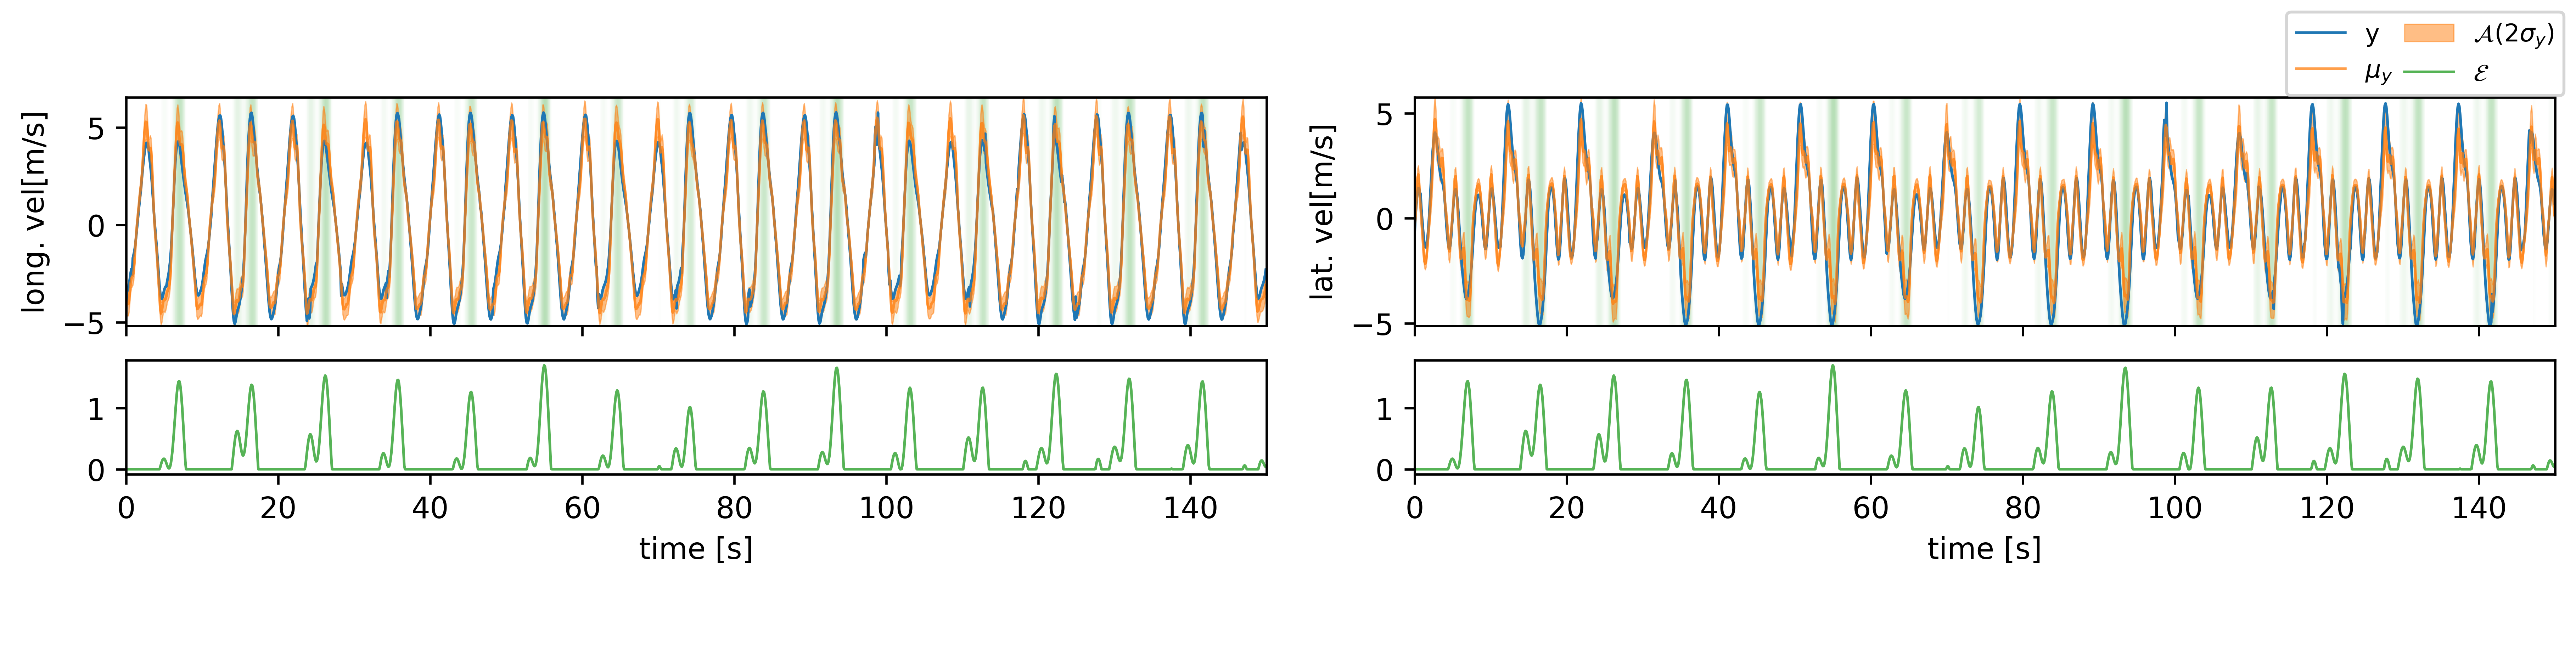
\includegraphics[width=\textwidth]{Experiments/figs/bb2_test.png}
    \caption{Test}
  \end{subfigure}
  
  \begin{subfigure}[b]{\textwidth}
    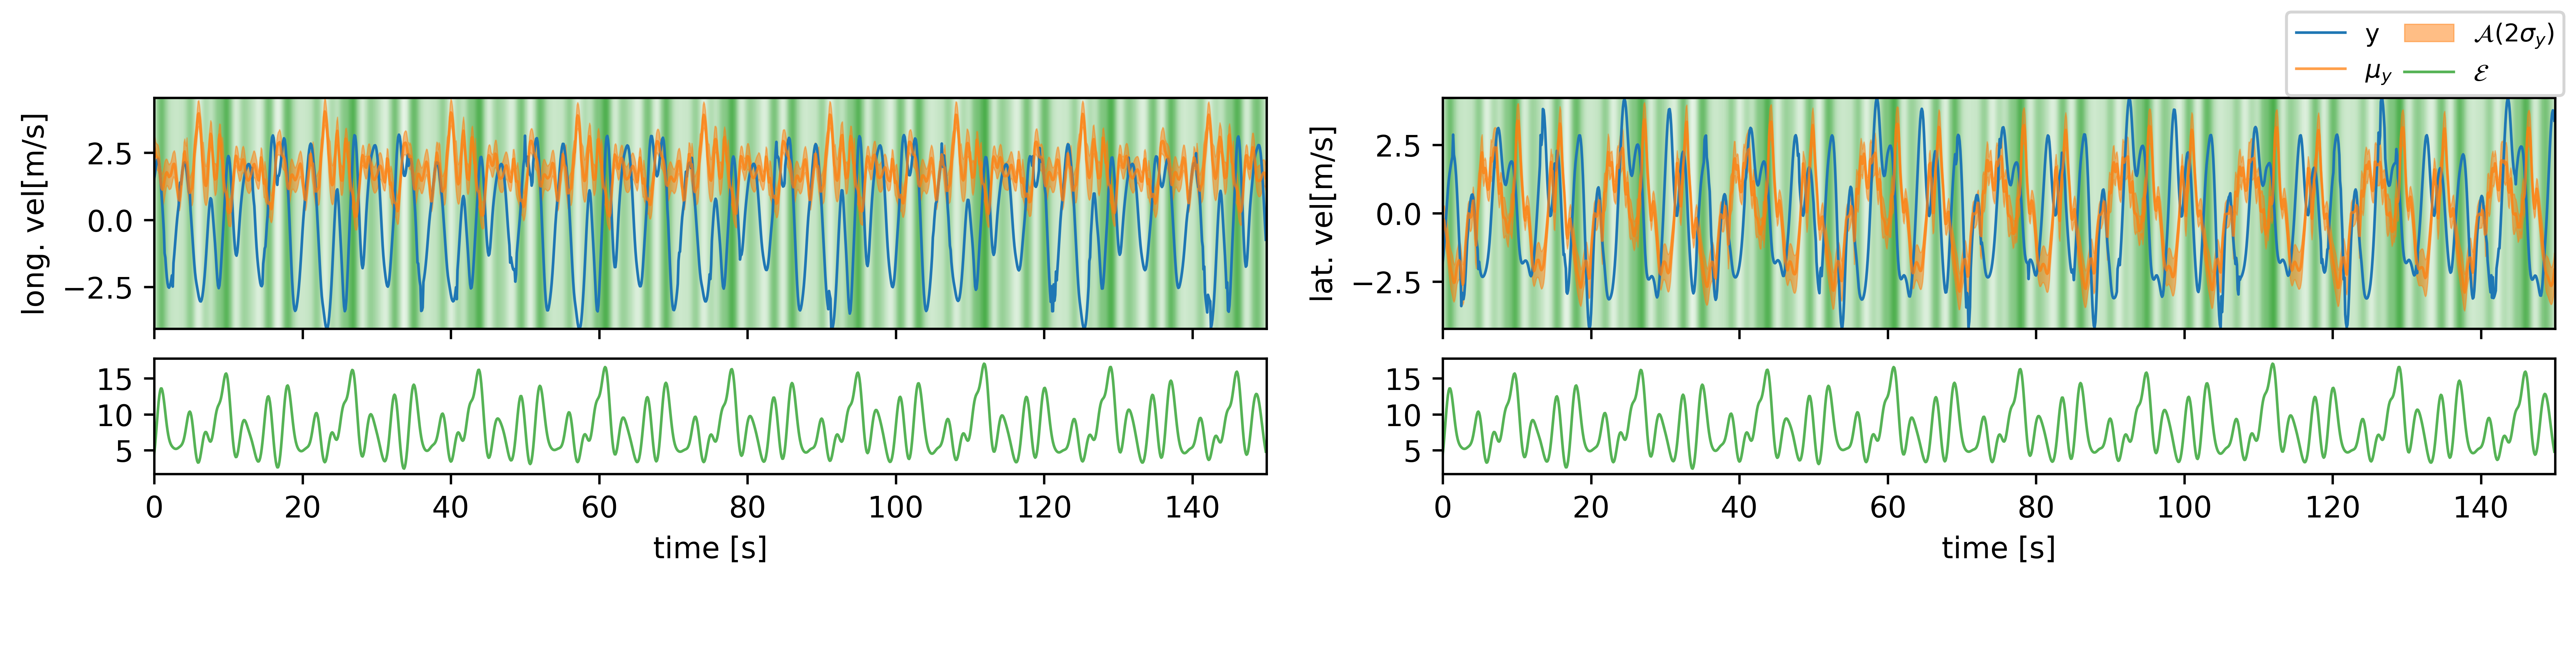
\includegraphics[width=\textwidth]{Experiments/figs/bb2_ood.png}
    \caption{OOD}
  \end{subfigure}
  
  \caption[Blackbird(2) prediction plots for C-RNN]{Blackbird(2) prediction plots for C-RNN. For plot description see \cref{sec:crnn_analysis}}
  \label{fig:bb2_run}
\end{figure}

\begin{table*}[h]
\centering
    \begin{tabular}{c  c  c   c  c }  
        \toprule
        Split & MAE & NLL & $\mathcal{A}$ & $\mathcal{E}$\\
        \midrule
        Test & 0.27(0.27, 0.32) & 0.22(0.14, 0.31) & 0.29(0.33, 0.33) &  -6.8\\
        OOD  &  1.12(1.2, 1) &  11.2(11.8, 10.6) & 0.35(0.6, 0.34)&  -3\\
        \midrule
    \end{tabular}
    \caption[Blackbird(2) C-RNN performance]{Blackbird(2) C-RNN performance.}
    \label{tbl:bb2_CRNN}
\end{table*}


\cref{fig:bb2_run} shows a flight sequence with the model predictions for a test and an OOD input. We can see from the plots that the model performs significantly worse on the OOD sequence. The epistemic uncertainty is much higher on the OOD input. \Cref{tbl:bb2_CRNN} shows the basic perfomance results. We the MAE for the test split is 0.27, and for the OOD split it is 1.15. The NLL of the test split is 0.22, for the OOD split it is 11.2. Thus the numbers show a significant decrease in performance between the splits. The average aleatoric uncertainty for the test split is 0.29, for the OOD split is 0.35. This already suggests that the aleatoric uncertainty does capture the increase in errors the model sees over the OOD data. The average epistemic uncertainty however goes from -6.8 over the test split, to -3 over the OOD split. This gives hope that the epistemic uncertainty captures the large errors the model commits for OOD inputs. 

\begin{table*}[h]
\centering
    \begin{tabular}{c  c  c}  
        \toprule
        Uncertainty score & AUROC$\uparrow$ & FPR@95\%$\downarrow$\\
        \midrule
        Aleatoric($\mathcal{A}$) & 0.54  & 0.8\\
        Epistemic($\mathcal{E}$) & 0.8 &  0.56 \\
        \midrule
    \end{tabular}
    \caption{Blackbird(2) OOD discrimination power for MC dropout.}
    \label{tbl:bb2_discrimination}
\end{table*}

\Cref{tbl:bb2_discrimination} shows how well our uncertainties can discriminate between the two splits. We can see that the aleatoric uncertainty does slightly better than random with an AUROC of 0.54. The epistemic uncertainty has a better AUROC of 0.8, which means a random OOD input has probability 0.8 of having higher epistemic uncertainty than a test input. 

It is challenging to gauge how good or bad the AUROC of 0.8 is in this context. Again, to better judge the quality of the uncertainty estimates we look at the correlation between the uncertainties and the errors. \Cref{tbl:bb2_corr} show the correlations between our uncertainties and error scores. First we note that the aleatoric uncertainty correlates very well with the MAE on each split individually, with a roughly 0.9 Pearson correlation with the MAE for both the test and OOD splits individually. However, over the combined split, we see that the aleatoric uncertainty gives a weaker correlation of 0.7. This makes sense given the aleatoric uncertainty is on average the same for the test and OOD splits, while the MAE is more than four times larger over the OOD split. The epistemic uncertainty shows a strong correlation with the MAE over the individual splits and the combined split, with a Pearson correlation of 0.9 over the combined splits. Moreover, we also see a strong Pearson correlation of 0.83 with the Z-score over the combined splits, suggesting that the epistemic uncertainty does go up for errors which are not explained away by the epistemic uncertainty. 


\begin{table*}[h]
\centering
    \begin{tabular}{l l c c c c}  
        \toprule
        U. & Split & \multicolumn{2}{c}{MAE} & \multicolumn{2}{c}{$Zs$}\\
        \midrule
        & & $\rho \uparrow$ & $r \uparrow$ & $\rho \uparrow$ & $r \uparrow$ \\
        \multirow{3}{*}{$\mathcal{A}$} 
            & Test     & 0.9(0.92, 0.87) & 0.89(0.89, 0.89) & - & - \\  
            & OOD      & 0.91(0.92, 0.89) & 0.94(0.94, 0.93) & - & - \\  
            & Test+OOD & 0.7(0.7, 0.7) & 0.74(0.72, 0.76) & - & - \\ 

        \midrule
        \multirow{3}{*}{$\mathcal{E}$} 
            & Test     & 0.92  & 0.91 &  0.48  & 0.63 \\  
            & OOD      & 0.87 & 0.91 &  0.83 & 0.83 \\
            & Test+OOD & 0.90 & 0.91 &  0.83 & 0.79 \\ 

        \toprule
    \end{tabular}
    \caption[Blackbird(2) error-uncertainty correlation for C-RNN]{Blackbird(2) error-uncertainty correlation for C-RNN. For table description see \cref{sec:crnn_analysis}}
    \label{tbl:bb2_corr}
\end{table*}


The correlation between the epistemic and aleatoric uncertainty is 0.61, suggesting that there is some overlap in the information they capture. But the results from \cref{tbl:bb2_corr} and \cref{tbl:bb2_discrimination} show that the epistemic uncertainty provides some information that is not contained in the aleatoric uncertainty. Namely, distinguishing between the in/out-of-distribution inputs. Next we will evaluate the performance of MC dropout. 

\begin{figure}[htbp]
  \centering
    \begin{subfigure}[b]{\textwidth}
        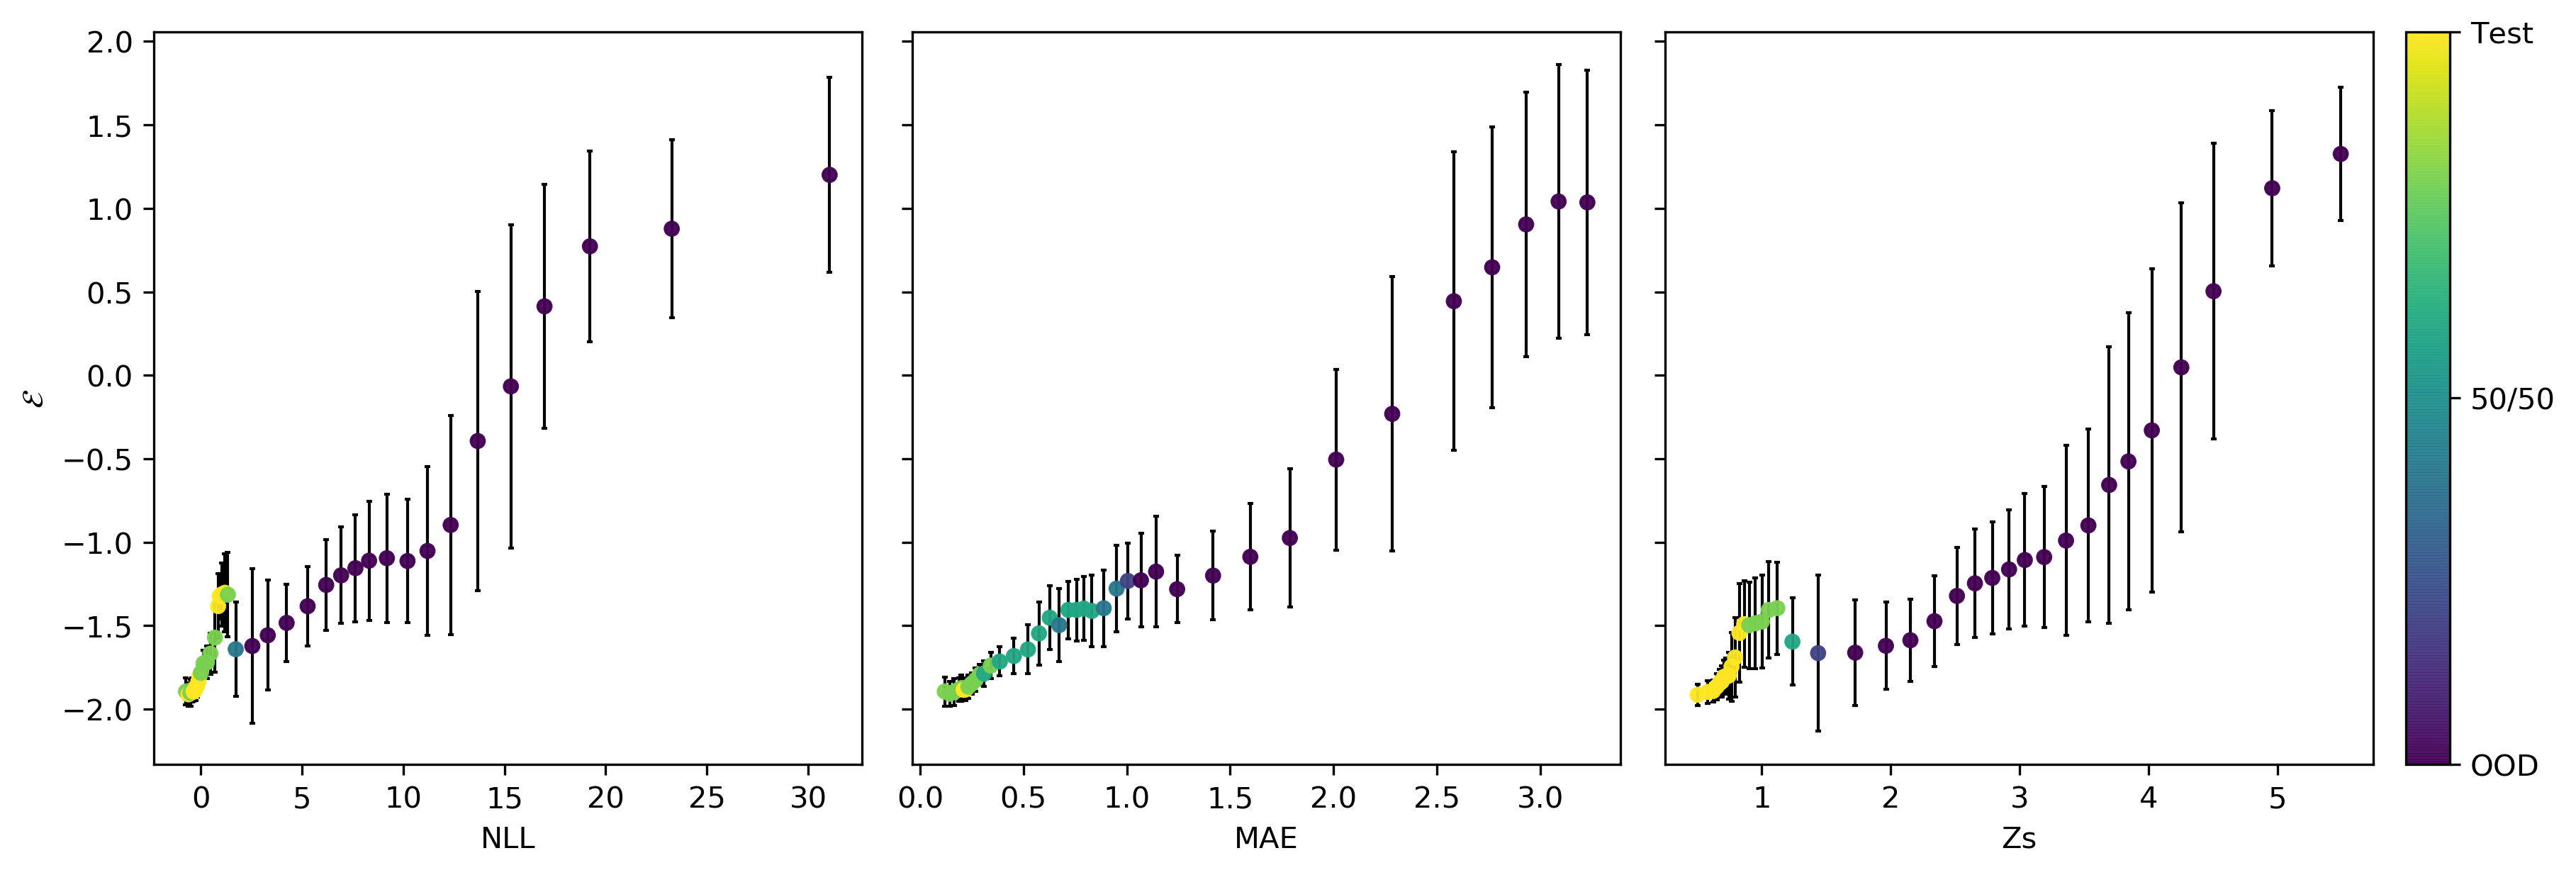
\includegraphics[width=\textwidth]{Experiments/figs/binned/bb2_crnn_epistemic.png}
        \caption{Binned diagonal plots for the epistemic uncertainty.}
    \end{subfigure}
    
    \begin{subfigure}[b]{\textwidth}
        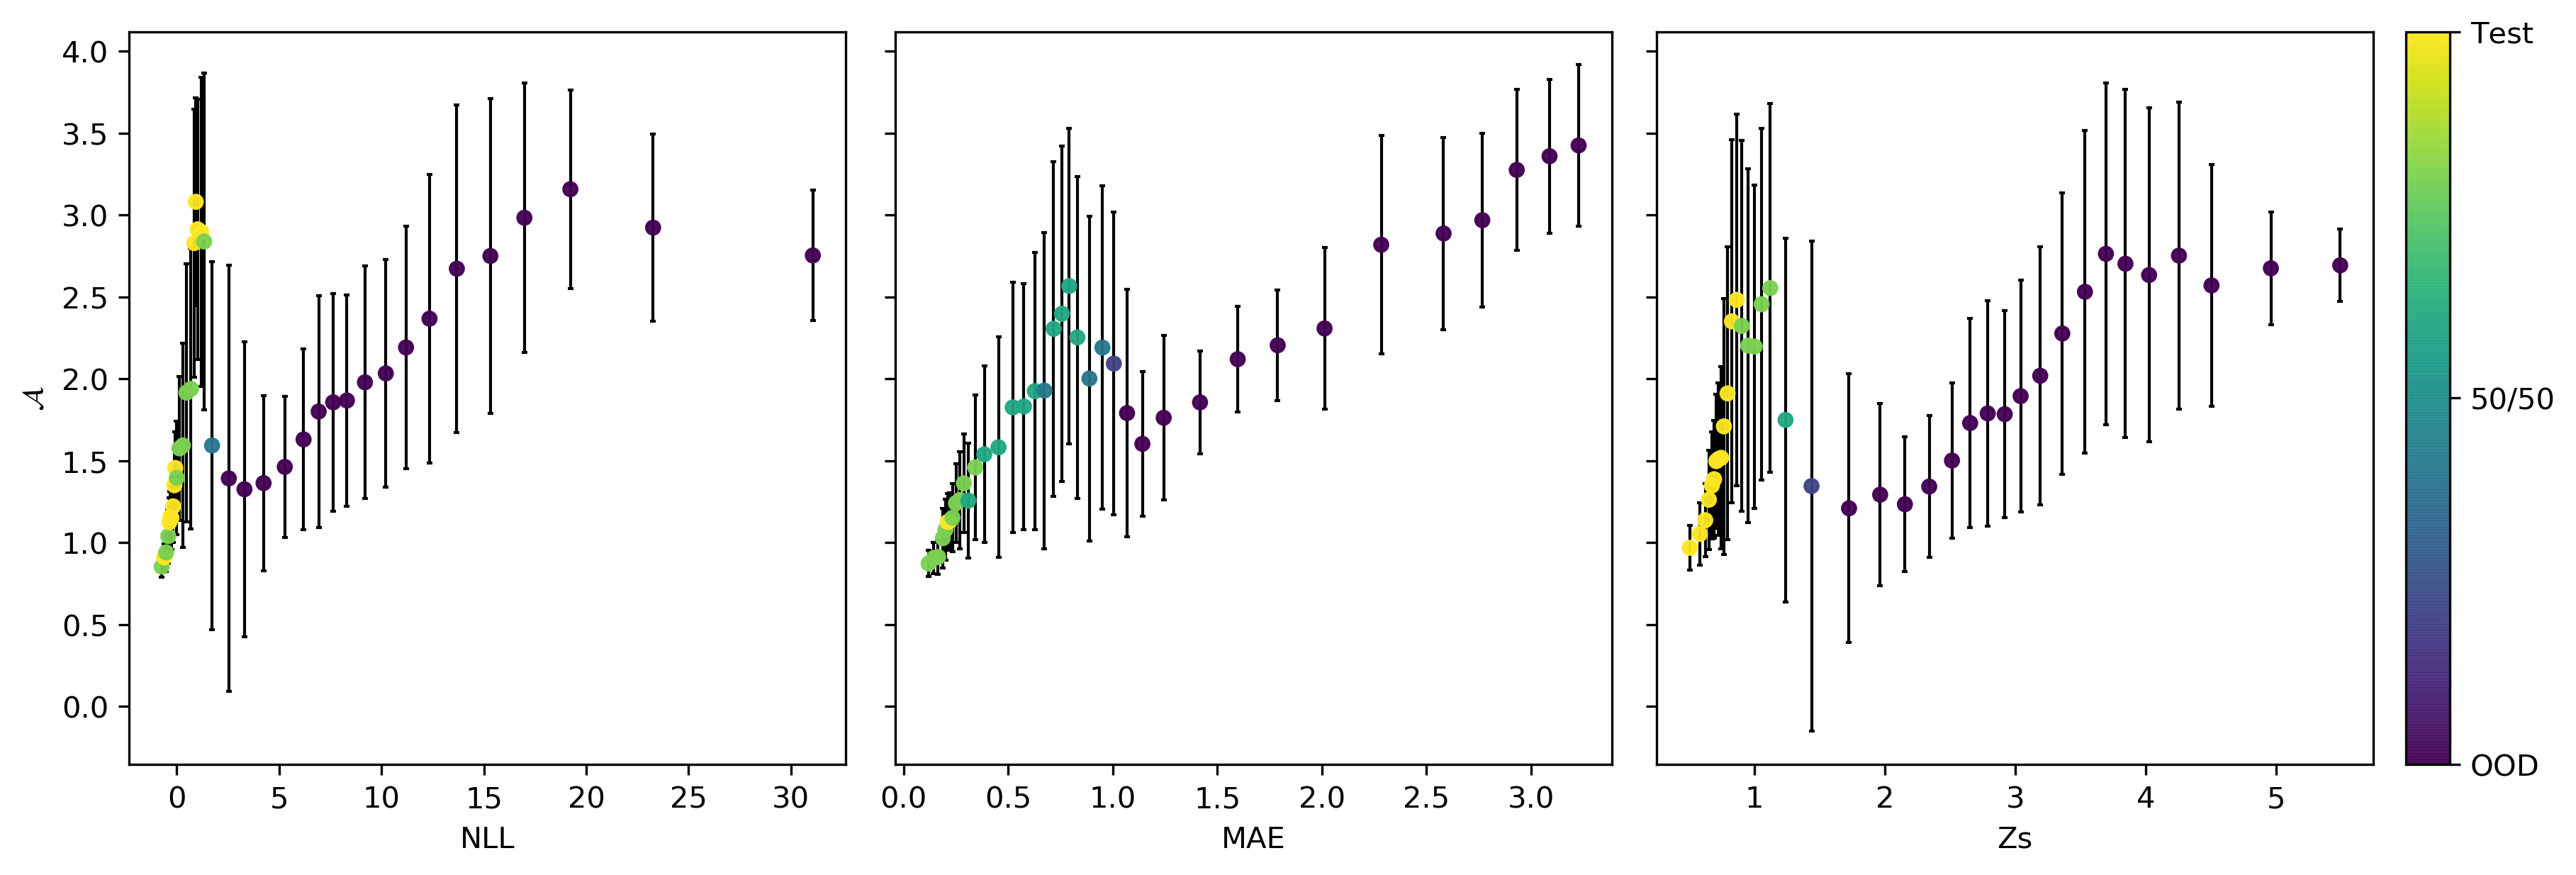
\includegraphics[width=\textwidth]{Experiments/figs/binned/bb2_crnn_aleatoric.png}
        \caption{Binned diagonal plots for the aleatoric uncertainty.}
  \end{subfigure}
    \caption[Blackbird(2) error-uncertainty diagonal plots for C-RNN]{Blackbird(2) error-uncertainty diagonal plots for C-RNN. For plot description see \cref{sec:crnn_analysis}}
    \label{fig:bb2_uncertainty_corr}
\end{figure}

\Cref{fig:bb2_uncertainty_corr} show the binned diagonal plots for errors versus uncertainties. The plots show that this split of Blackbird presents mixed results. Like the Revs results for C-RNN (\cref{fig:revs_uncertainty_corr}), the data seems to separated to a low error in distribution cluster, followed by a high error OOD tail. However, the pattern is not as clear.
Some of the bins in the two extremes seem to be mostly coming from a single split, but in the middle we see mixed bins. 
The aleatoric uncertainty exhibits the same dynamic we have seen on the Revs dataset(\cref{fig:revs_uncertainty_corr}), where it correlates well with the MAE in the beginning, then \emph{restarts} and correlates separately with the high error points. However, the pattern is not as strong here. 
The epistemic uncertainty correlates well with the errors and separates the in/out-of-distribution points, however not as strongly as we see on the Revs dataset. In the next section, we will see how dropout handles this case. 


\clearpage
\subsection{MC dropout analysis}

\begin{figure}[h]
  \centering
  
  \begin{subfigure}[b]{\textwidth}
    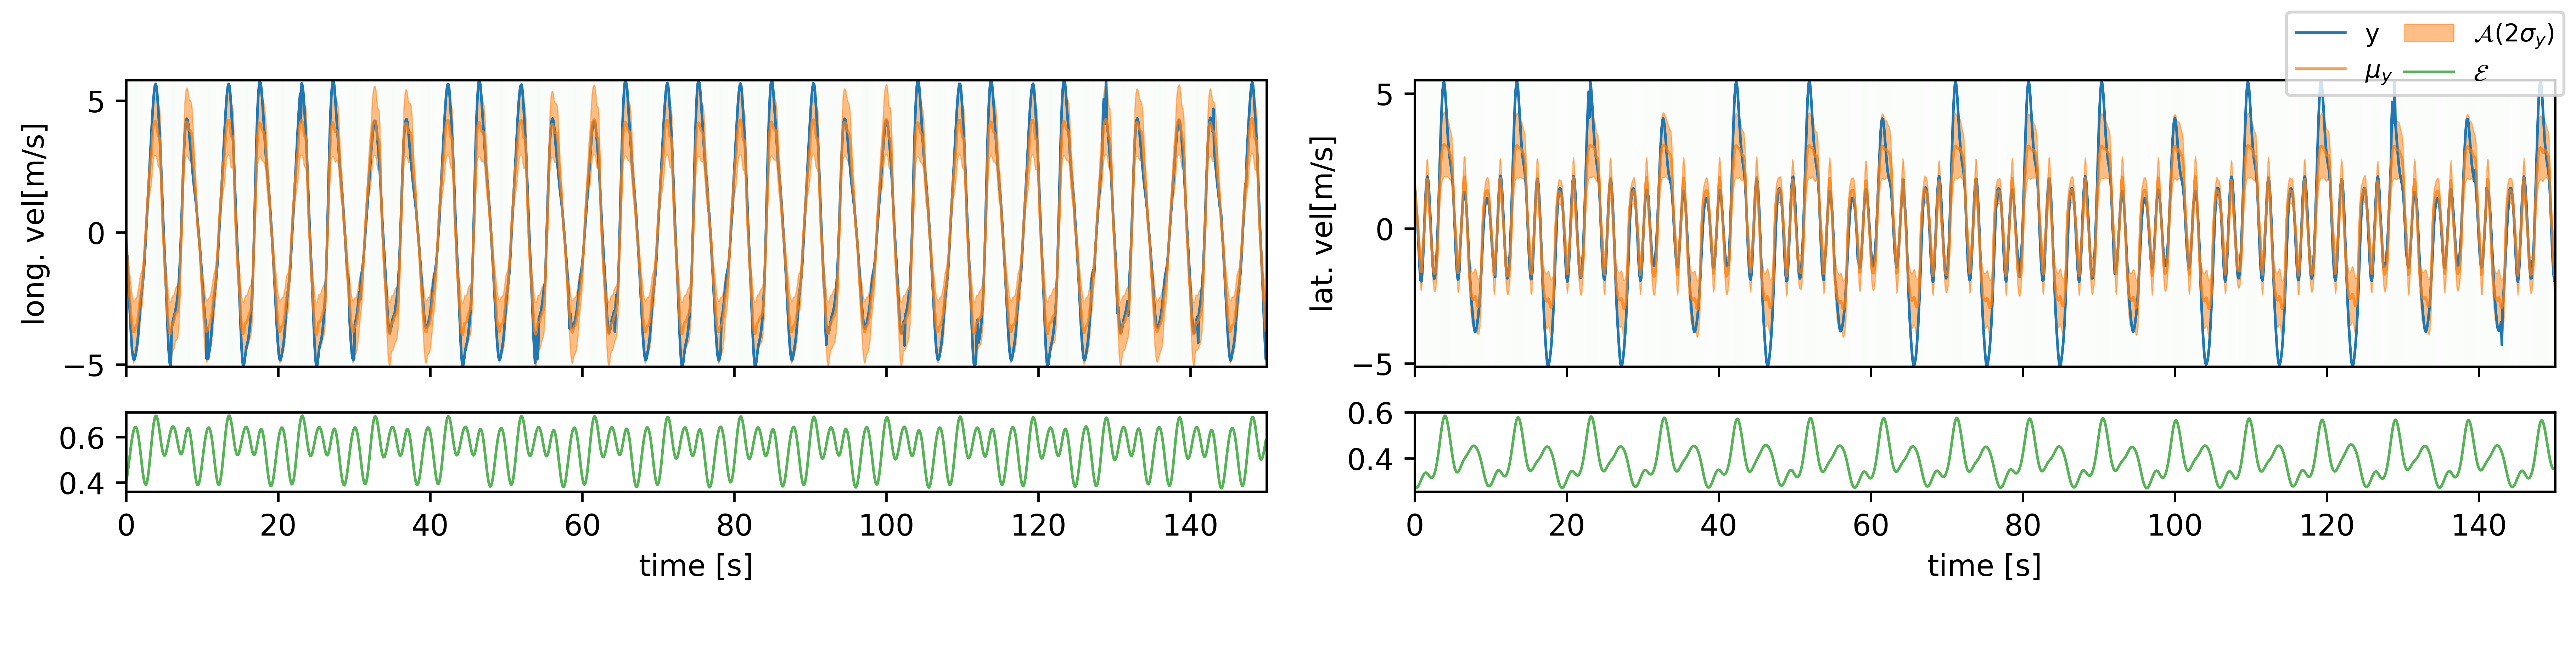
\includegraphics[width=\textwidth]{Experiments/figs/bb2_dropout_test.png}
    \caption{Test}
  \end{subfigure}
  
  \begin{subfigure}[b]{\textwidth}
    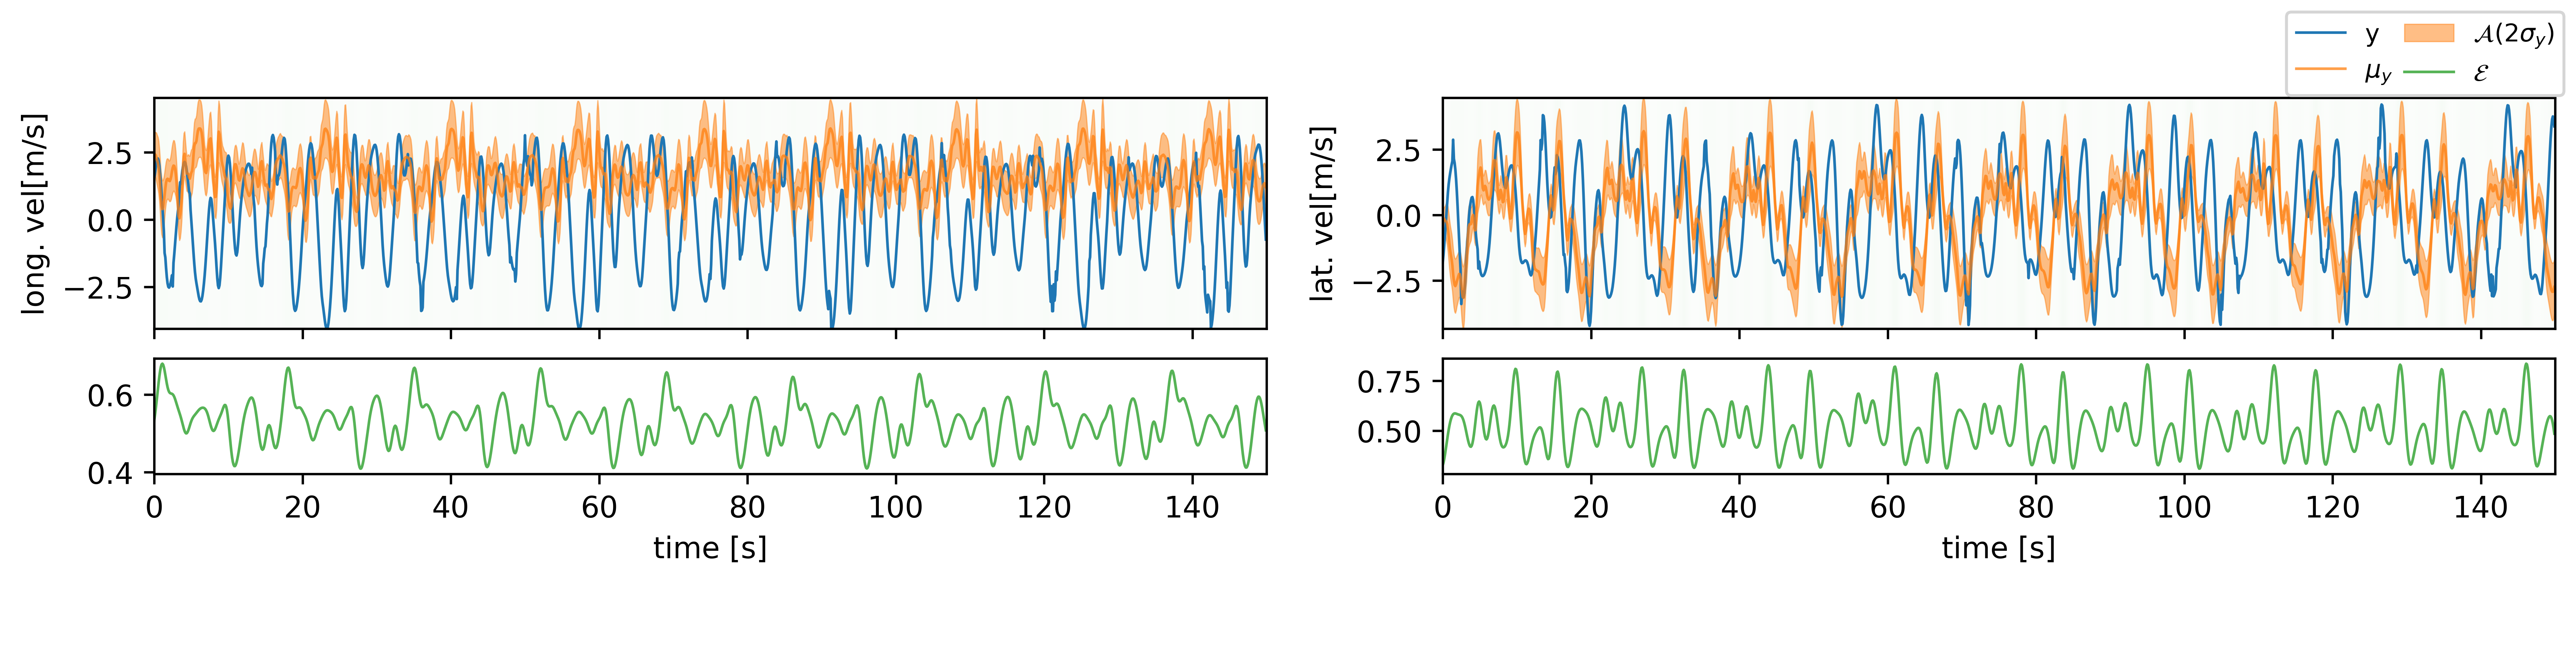
\includegraphics[width=\textwidth]{Experiments/figs/bb2_dropout_ood.png}
    \caption{OOD}
  \end{subfigure}
  
  \caption[Blackbird(2) prediction plots for MC dropout]{Blackbird(2) prediction plots for MC dropout. For plot description see \cref{sec:crnn_analysis}}
  \label{fig:bb2_dropout_run}
\end{figure}

\begin{table*}[h]
\centering
    \begin{tabular}{c  c  c  c  c }  
        \toprule
        Split & MAE & NLL & $\mathcal{A}$ & $\mathcal{E}$\\
        \midrule
        Test & 0.27(0.26, 0.29) & 0.22(0.19, 0.25) & 0.42(0.42, 0.41) &  0.28(0.28, 0.28)\\
        OOD  &  1.1(1.14, 1) &  7.3(7.3, 7.4) & 0.33(0.35, 0.32)&  0.28(0.3, 0.26)\\
        \midrule
    \end{tabular}
    \caption{Blackbird(2) MC dropout performance.}
    \label{tbl:bb2_dropout}
\end{table*}



\Cref{fig:bb2_dropout_run} shows a flight sequence with the model predictions for a test and an OOD sequence for the MC dropout model. A familiar patter emerges, the model visibly performs worse on the OOD sample, yet the epistemic and aleatoric uncertainties don't seem to capture that decrease in accuracy. \Cref{tbl:bb2_dropout} contains the performance measures. We can see the MAE and NLL increase from 0.27 and 0.22 respectively over the test split, to 1.1 and 7.3 over the OOD split. However, the epistemic and aleatoric uncertainties show no increase with the aleatoric uncertainty being actually lower on the OOD split. \Cref{tbl:bb2_dropout_discrimination} confirms that neither the epistemic or aleatoric uncertainty from MC dropout provides a useful signal for detecting OOD inputs, with AUROC scores around 0.5 similar to the expected performance of a random classifier. 


\begin{table*}[h]
\centering
    \begin{tabular}{c  c  c}  
        \toprule
        Uncertainty score & AUROC$\uparrow$ & FPR@95\%$\downarrow$\\
        \midrule
        Aleatoric($\mathcal{A}$) & 0.48  & 0.82\\
        Epistemic($\mathcal{E}$) & 0.48 &  0.81 \\
        \midrule
    \end{tabular}
    \caption{blackbird(2) OOD discrimination power for MC dropout.}
    \label{tbl:bb2_dropout_discrimination}
\end{table*}

\Cref{tbl:bb2_dropout_corr} shows the correlations between the uncertainties and the errors for MC dropout. We see that both uncertainties show strong correlation with the MAE for the individual splits, but not for the combined split. The epistemic uncertainty only correlates weakly with the Z-score. Moreover, note that the performance of both uncertainties is very similar overall. 


\begin{table*}[h]
\centering
    \begin{tabular}{l l c c c c}  
        \toprule
        U. & Split & \multicolumn{2}{c}{MAE} & \multicolumn{2}{c}{$Zs$}\\
        \midrule
        & & $\rho \uparrow$ & $r \uparrow$ & $\rho \uparrow$ & $r \uparrow$ \\
        \multirow{3}{*}{$\mathcal{A}$} 
            & Test     & 0.84(0.88, 0.8) & 0.89(0.89, 0.88) & - & - \\  
            & OOD      & 0.89(0.94, 0.85) & 0.91(0.92, 0.9) & - & - \\  
            & Test+OOD & 0.49(0.51, 0.46) & 0.49(0.51, 0.47) & - & - \\ 

        \midrule
        \multirow{3}{*}{$\mathcal{E}$} 
            & Test     & 0.84(0.87, 0.8)  & 0.87(0.87, 0.87) & 0.43(0.42, 0.44) & 0.45(0.43, 0.46) \\  
            & OOD      & 0.91(0.93, 0.88) & 0.92(0.93, 0.91) & 0.54(0.67, 0.41) & 0.58(0.67, 0.5) \\
            & Test+OOD & 0.69(0.72, 0.65) & 0.69(0.72, 0.65) & 0.31(0.41, 0.2) & 0.3(0.39, 0.21) \\ 

        \toprule
    \end{tabular}
    \caption[Blackbird(2) error-uncertainty correlation for MC dropout]{Blackbird(2) error-uncertainty correlation for MC dropout. For table description see \cref{sec:crnn_analysis}}
    \label{tbl:bb2_dropout_corr}
\end{table*}

We compute the correlation between the aleatoric and epistemic uncertainty and obtain a Pearson coefficient of 0.94. This shows that for MC dropout both uncertainties give us mostly the same information. Again this was also found empirically by \cite{kendall2017uncertainties}. 

\begin{figure}[htbp]
  \centering
    \begin{subfigure}[b]{\textwidth}
        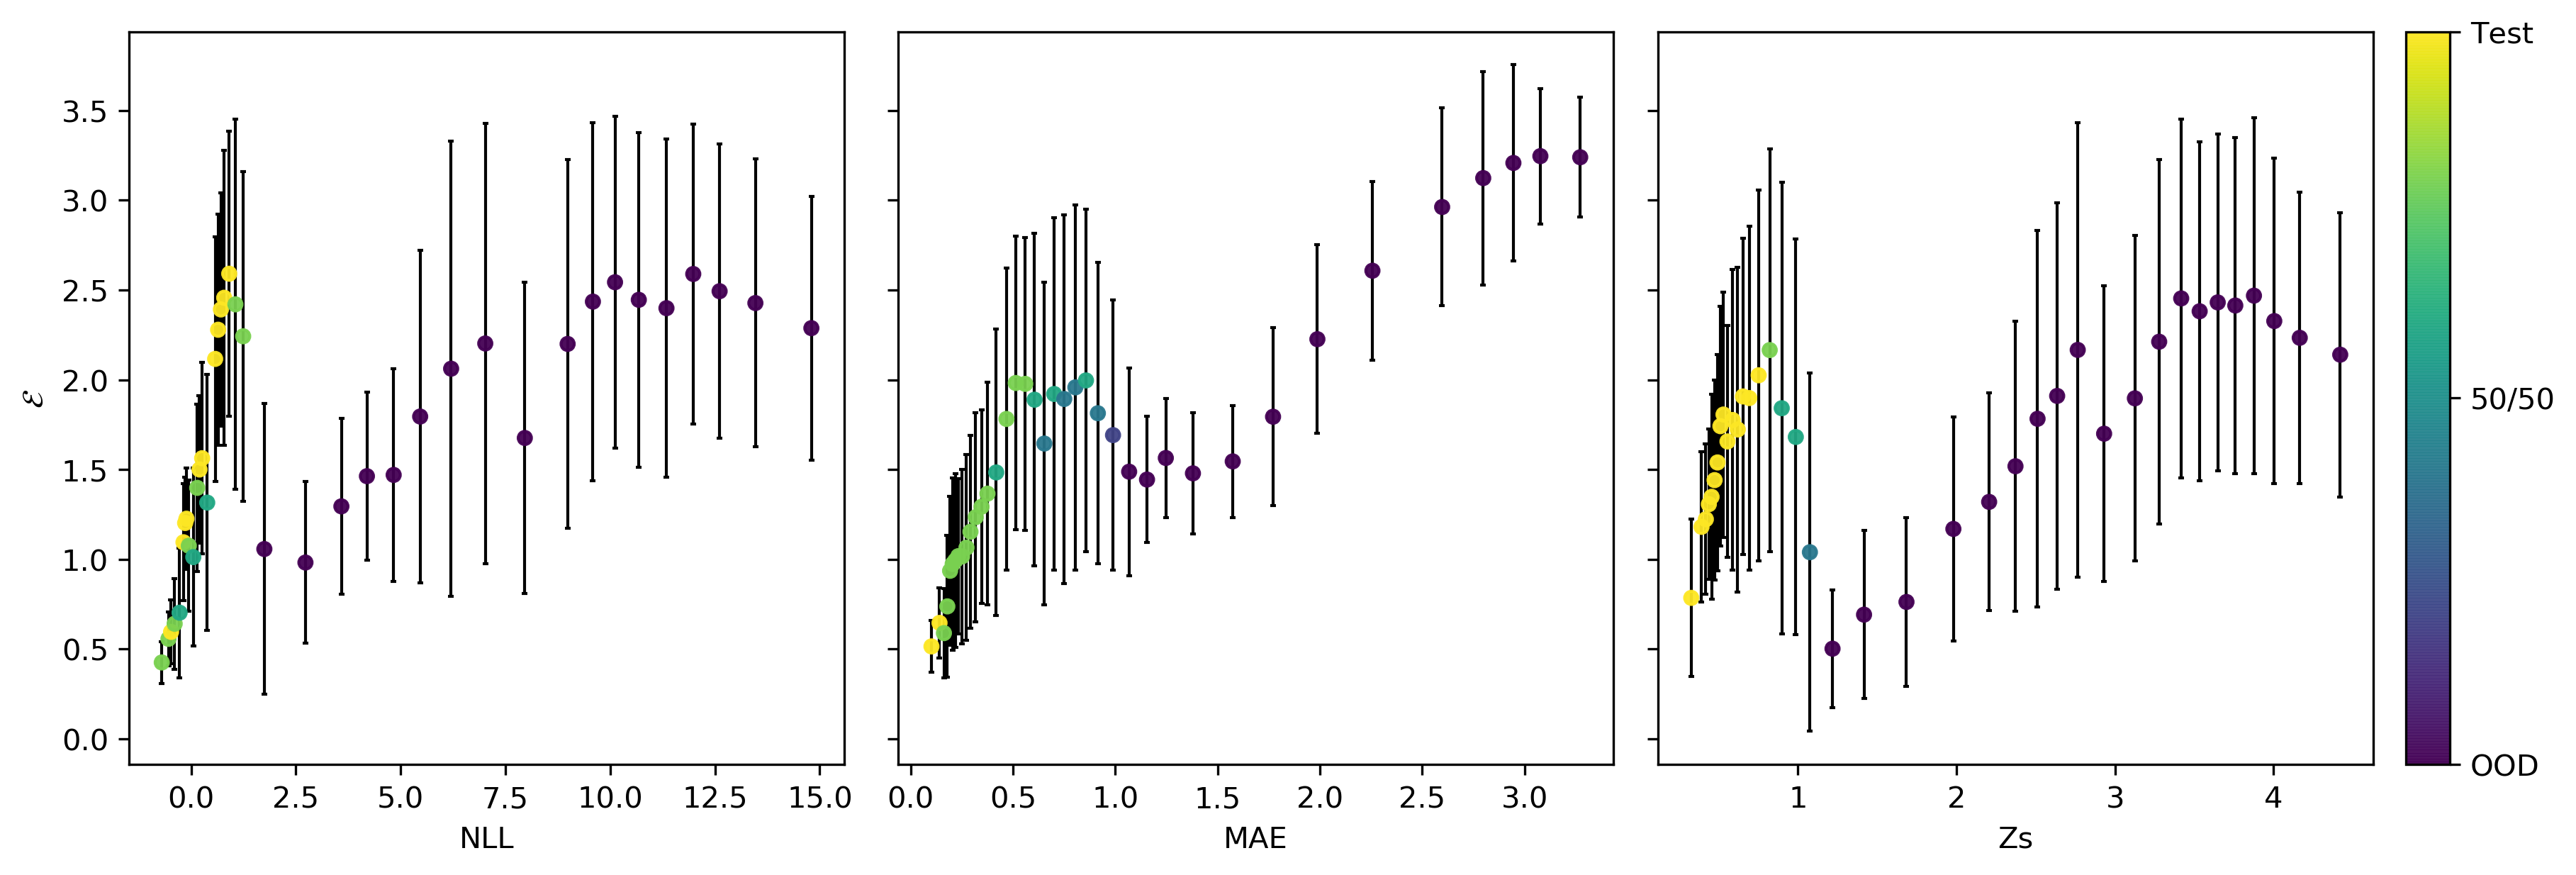
\includegraphics[width=\textwidth]{Experiments/figs/binned/bb2_dropout_epistemic.png}
        \caption{Binned diagonal plots for the epistemic uncertainty.}
    \end{subfigure}
    
    \begin{subfigure}[b]{\textwidth}
        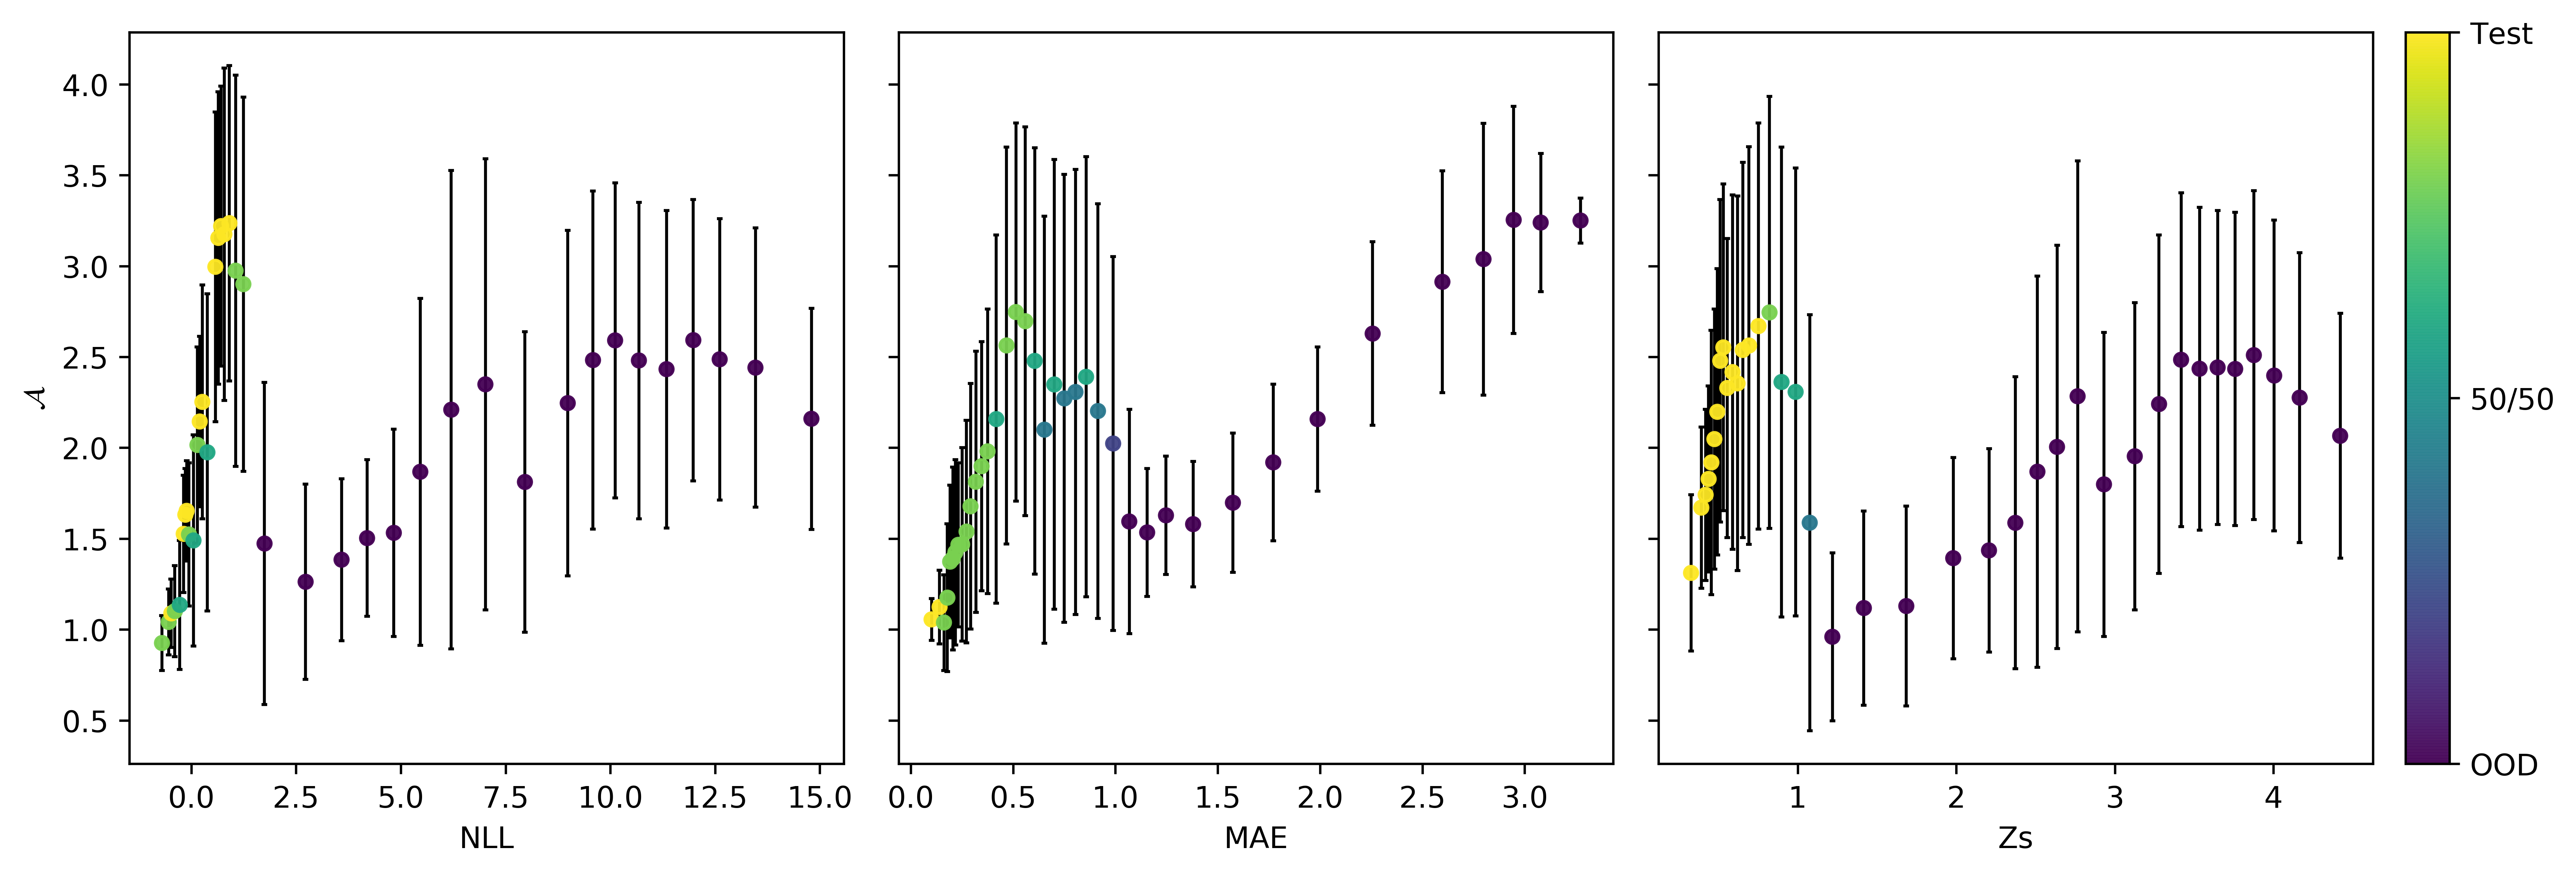
\includegraphics[width=\textwidth]{Experiments/figs/binned/bb2_dropout_aleatoric.png}
        \caption{Binned diagonal plots for the aleatoric uncertainty.}
  \end{subfigure}
    \caption[Blackbird(2) error-uncertainty diagonal plots for MC dropout]{Blackbird(2) error-uncertainty diagonal plots for MC dropout. For plot description see \cref{sec:crnn_analysis}}
    \label{fig:bb2_dropout_uncertainty_corr}
\end{figure}

\Cref{fig:bb2_dropout_uncertainty_corr} shows the binned diagonal plots for errors versus uncertainties. For both uncertainties, we see the familiar pattern of the uncertainty correlating with the error in the beginning then \emph{resetting} and correlated separately with the tail. The plots also give visual testimony to the notion that MC dropout's epistemic uncertainty overlaps highly with the aleatoric uncertainty in terms of information about the errors. Comparing the plots here with the ones for C-RNN(\cref{fig:bb2_uncertainty_corr}), we can see that C-RNN's epistemic uncertainty gives information that MC dropout does not capture. Not just for better separating in/out-of-distribution data, but also  a stronger correlation with the error for the OOD inputs. We will distill the key findings for Blackbird(2) in the next section. 

\clearpage
\subsection{Key findings}

In general, the findings of this section go along the same lines of the findings in \cref{sec:revs_results}. We find that 

\begin{itemize}
    \item The epistemic uncertainty from C-RNN is useful in separating the in/out-of-distribution inputs.
    \item The epistemic uncertainty from MC dropout is of no use in separating the in/out-of-distribution inputs.
    \item For C-RNN the epistemic and aleatoric uncertainties are moderately correlated, but the epistemic uncertainty provides more information. 
    \item For MC dropout the aleatoric and epistemic uncertainties are strongly correlated and seem to provide the same information. 
\end{itemize}{}


In \cref{tbl:bb2_comparison} we have a summary of the key metrics for comparison of C-RNN and MC dropout. The table supports our key findings, we can see that C-RNN gets an AUROC of 0.8, whereas MC dropout gets an AUROC of 0.48, showing that C-RNN has some success in separating in/out-of-distribution inputs and MC dropout is performing as well as random guessing. MC dropout has high correlation between epistemic uncertainty over each split individually with 0.84 and 0.91 Pearson coefficient for the test and OOD splits respectively, but an 0.69 Pearson coefficient for the combined splits, whereas C-RNN has a Pearson coefficient of 0.9 over the combined splits.  

\begin{table*}[h]
\centering
    \begin{tabular}{l l c c c c c}  
        \toprule
        Model & split & MAE & NLL & $\rho$(MAE vs $\mathcal{E}$) &
        $\rho$(Z-score vs $\mathcal{E}$) & AUROC($\mathcal{E}$)\\
        \midrule
        \multirow{3}{*}{C-RNN} 
            & Test     & 0.27 & 0.22 & 0.92 & 0.48 & - \\  
            & OOD      & 1.12 & 11.2 & 0.87 & 0.83 & -\\  
            & Test+OOD & 0.7  & 5.7  & 0.9  & 0.83 & 0.8\\ 

        \midrule
        \multirow{3}{*}{MC dropout} 
            & Test     & 0.27 & 0.22 & 0.84  & 0.43 & - \\  
            & OOD      & 1.1 & 7.3   & 0.91  & 0.54 & -\\  
            & Test+OOD & 0.69 & 3.7  & 0.69  & 0.31 & 0.48\\ 

        \toprule
    \end{tabular}
    \caption{Blackbird(2) key results for comparison of C-RNN and MC dropout.}
    \label{tbl:bb2_comparison}
\end{table*}

So far, we have conducted experiments over two datasets and three different settings overall. We saw numerous patterns persist. In the next section, we will distill the patterns we found in all our experiments.

